\documentclass[border={0.1cm 0.1cm 0.1cm 0.1cm}]{standalone}  %E,S,W,N

\usepackage{amssymb}
\usepackage{amsmath}
\usepackage{tikz}
\usetikzlibrary{calc}	%for centerarc

\def\centerarc[#1](#2)(#3:#4:#5) {\draw[#1] ($(#2)+({#5*cos(#3)},{#5*sin(#3)})$) arc (#3:#4:#5);}
%polar coordinates: ({4*cos(90)},{4*sin(90)})

%Phase portrait of the Ashtanga Yoga Sutras, by Blake Victor (@intendtogether)

\begin{document}
	
	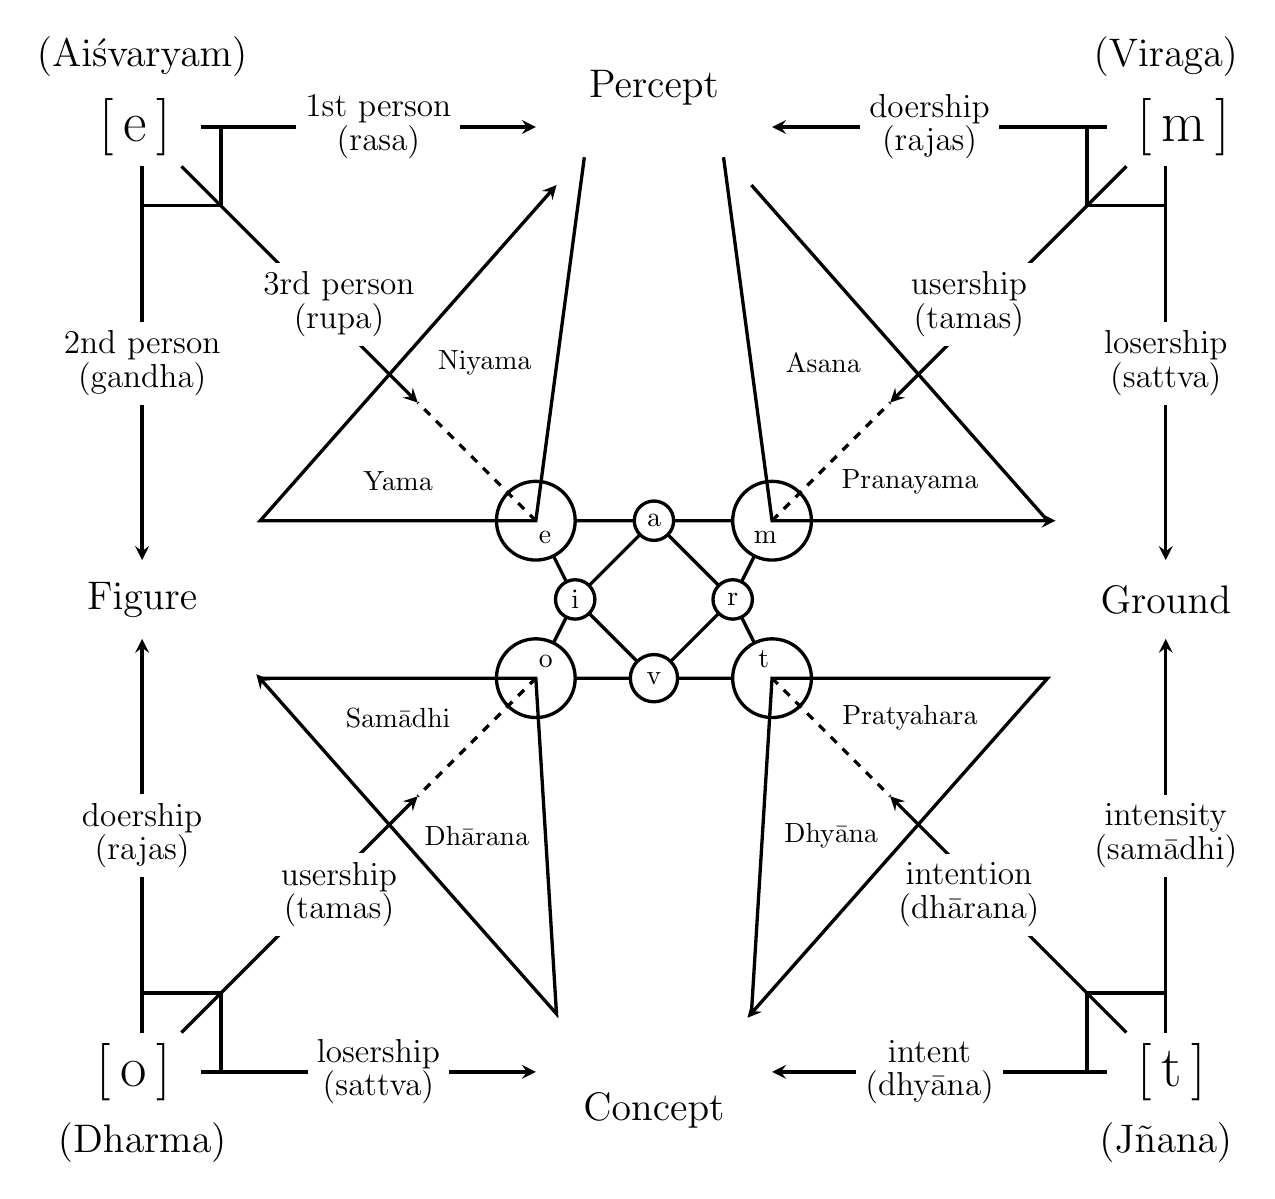
\begin{tikzpicture}[very thick]	
	\draw (0,1)--(1,0)--(0,-1)--(-1,0)--cycle;
	\draw (-1.5,-1)--(-1,0)--(-1.5,1)--(0,1)--(1.5,1)--(1,0)--(1.5,-1)--(0,-1)--cycle;
	%
	\filldraw[fill=white] (0,1) circle (0.25cm) node {a};
	\filldraw[fill=white] (0,-1) circle (0.3cm) node {v};
	\filldraw[fill=white] (-1,0) circle (0.25cm) node {i};
	\filldraw[fill=white] (1,0) circle (0.25cm) node {r};
	%
	\filldraw[fill=white,below left] (1.5,1) circle (0.5cm) node[xshift=0.2cm] {m};
	\filldraw[fill=white,below right] (-1.5,1) circle (0.5cm) node[xshift=-0.1cm] {e};
	\filldraw[fill=white,above right] (-1.5,-1) circle (0.5cm) node[xshift=-0.1cm] {o};
	\filldraw[fill=white,above left] (1.5,-1) circle (0.5cm) node[xshift=0.1cm] {t};
	
	%DIAGONAL ARROWS
	\draw[dashed] (-1.5,1)--(-3,2.5);	
	\draw[<-,>=stealth] (-3,2.5)--++(-3,3) node[above left] {\huge [$\,$e$\,$]};
	%
	\draw[dashed] (1.5,1)--(3,2.5);
	\draw[<-,>=stealth] (3,2.5)--++(3,3) node[above right] {\huge [$\,$m$\,$]};
	%
	\draw[dashed] (1.5,-1)--(3,-2.5);
	\draw[<-,>=stealth] (3,-2.5)--++(3,-3) node[below right] {\huge [$\,$t$\,$]};
	%
	\draw[dashed] (-1.5,-1)--(-3,-2.5);
	\draw[<-,>=stealth] (-3,-2.5)--++(-3,-3) node[below left] {\huge [$\,$o$\,$]};
	
	%OUTER LABELS
	\node at (-6.5,0) {\Large Figure};		
	\centerarc[](-6.5,0)(90+15:270-15:1.25)
	\centerarc[](-6.5,0)(-90+15:90-15:1.25)
	%
	\node at (6.5,0) {\Large Ground};
	\centerarc[](6.5,0)(90+15:270-15:1.25)
	\centerarc[](6.5,0)(-90+15:90-15:1.25)
	%
	\node at (0,6.5) {\Large Percept};
	\centerarc[](0,6.5)(-90+45:270-45:1.25)
	%
	\node at (0,-6.5) {\Large Concept};
	\centerarc[](0,-6.5)(90+45:405:1.25)
	%
	\node[above] at (-6.5,6.5) {\Large (Ai\'{s}varyam)};
	\node[below] at (-6.5,-6.5) {\Large (Dharma)};
	\node[above] at (6.5,6.5) {\Large (Viraga)}; %detachment
	%\node[above] at (6.5,6.5) {\Large (\'{S}akti)};
	%\node[right] at (7.25,6) {\Large (raga)};
	%\node[right] at (6.65,5) {\Large (prakrti)};
	\node[below] at (6.5,-6.5) {\Large (J\~{n}ana)};
	
	%CORNER ARROWS
	\draw[->,>=stealth] (-6.5,-5.5)--++(0,5);
	\draw[->,>=stealth] (-6.5,5.5)--++(0,-5);
	\draw[->,>=stealth] (6.5,-5.5)--++(0,5);
	\draw[->,>=stealth] (6.5,5.5)--++(0,-5);
	%
	\draw[->,>=stealth] (-5.75,-6)--++(4.25,0);
	\draw[->,>=stealth] (5.75,-6)--++(-4.25,0);
	\draw[->,>=stealth] (-5.75,6)--++(4.25,0);
	\draw[->,>=stealth] (5.75,6)--++(-4.25,0);
	%
	\node[align=center,fill=white] at (-6.5,-3) {\large doership \\ \large (rajas)};
	\node[align=center,fill=white] at ( 6.5,-3) {\large intensity \\ \large (sam\={a}dhi)};
	\node[align=center,fill=white] at (-6.5, 3) {\large 2nd person \\ \large (gandha)};
	\node[align=center,fill=white] at ( 6.5, 3) {\large losership \\ \large (sattva)}; %or: continence
	%
	\node[align=center,fill=white] at (-3.5,-6) {\large losership \\ \large (sattva)};
	\node[align=center,fill=white] at ( 3.5,-6) {\large intent \\ \large (dhy\={a}na)};
	\node[align=center,fill=white] at (-3.5, 6) {\large 1st person \\ \large (rasa)};
	\node[align=center,fill=white] at ( 3.5, 6) {\large doership \\ \large (rajas)}; %or: salience
	%
	\node[align=center,fill=white] at (-4,-3.75) {\large usership \\ \large (tamas)};
	\node[align=center,fill=white] at ( 4,-3.75) {\large intention \\ \large (dh\={a}rana)};
	\node[align=center,fill=white] at (-4, 3.75) {\large 3rd person \\ \large (rupa)};
	\node[align=center,fill=white] at ( 4, 3.75) {\large usership \\ \large (tamas)}; %or: pertinence
	
	%TRIANGLES
	%\centerarc[](0,6.5)(-90+45:270-45:1.25)
	\draw[->,>=stealth] ({1.25*cos(270-45)},{6.5+1.25*sin(270-45)})--(-1.5,1)--(-5,1)-- ({1.75*cos(270-45)},{6.5+1.75*sin(270-45)});
	\draw[->,>=stealth] ({1.25*cos(270+45)},{6.5+1.25*sin(270+45)})--(1.5,1)--(5.1,1);
	\draw (5,1)--({1.75*cos(270+45)},{6.5+1.75*sin(270+45)});
	\draw[->,>=stealth] (-5,-1)--(-1.5,-1)--({1.75*cos(90+45)},{-6.5+1.75*sin(90+45)})--(-5-.05,-1+.05);
	\draw[->,>=stealth] ({1.75*cos(90-45)},{-6.5+1.75*sin(90-45)})--(1.5,-1)--(5,-1)-- ({1.75*cos(90-45)-0.05},{-6.5+1.75*sin(90-45)-0.05});
	
	%CORNERS
	\draw (-6.5,-5)--(-5.5,-5)--(-5.5,-6);
	\draw ( 6.5,-5)--( 5.5,-5)--( 5.5,-6);
	\draw ( 6.5, 5)--( 5.5, 5)--( 5.5, 6);
	\draw (-6.5, 5)--(-5.5, 5)--(-5.5, 6);
	
	%INNER LABELS
	\node at (-3.25,1.5) {Yama};
	\node at (-2.15,3) {Niyama};
	%
	\node at (3.25,1.5) {Pranayama};
	\node at (2.15,3) {Asana};
	%
	\node at (-3.25,-1.5) {Sam\={a}dhi};
	\node at (-2.25,-3) {Dh\={a}rana};
	%
	\node at (3.25,-1.5) {Pratyahara};
	\node at (2.25,-3) {Dhy\={a}na};
	\end{tikzpicture}
	
\end{document}